\documentclass[11pt,a4paper]{article}

\usepackage[margin=0.82in]{geometry}
\usepackage{amsmath,amssymb}
\usepackage{booktabs}
\usepackage{graphicx}
\usepackage{microtype}
\usepackage{enumitem}
\usepackage{caption}
\usepackage{subcaption}
\usepackage{tikz}
\usepackage{etoolbox}
\usepackage[hidelinks]{hyperref}
\usepackage[T1]{fontenc}

\usetikzlibrary{arrows.meta,positioning}
\setlength{\parindent}{0pt}
\setlength{\parskip}{4pt}
\setlist{nosep,leftmargin=*}
\captionsetup{font=small}
\graphicspath{{../outputs/}}
% Generated by scripts/summarize_results.py; do not edit by hand.
\newcommand{\CifarAvailable}{yes}
\newcommand{\CifarTrainN}{256}
\newcommand{\CifarTestN}{1000}
\newcommand{\CifarRootTrain}{91.02}
\newcommand{\CifarRootTest}{29.50}
\newcommand{\CifarRootTrainLoss}{0.611}
\newcommand{\CifarRootTestLoss}{2.041}
\newcommand{\CifarFinalTrain}{100.00}
\newcommand{\CifarFinalTest}{29.80}
\newcommand{\CifarFinalTrainLoss}{0.404}
\newcommand{\CifarFinalTestLoss}{2.148}
\newcommand{\CifarTrainGain}{8.98}
\newcommand{\CifarTestGain}{0.30}
\newcommand{\CifarNodes}{11}
\newcommand{\CifarParameters}{128,176}
\newcommand{\CifarParameterGrowth}{61.1}
\newcommand{\CifarRetainedNodes}{9}
\newcommand{\CifarPrunedParameters}{119,340}
\newcommand{\CifarPruningReduction}{6.9}
\newcommand{\CifarPrunedTrain}{99.22}
\newcommand{\CifarPrunedTest}{29.70}
\newcommand{\CifarInterpolates}{yes}
\newcommand{\CifarRootEpoch}{20}
\newcommand{\CifarRootTarget}{85.00}
\newcommand{\CifarPruneAccuracy}{99.00}
\newcommand{\PetsAvailable}{yes}
\newcommand{\PetsTrainN}{256}
\newcommand{\PetsTestN}{256}
\newcommand{\PetsRootTrain}{91.41}
\newcommand{\PetsRootTest}{68.75}
\newcommand{\PetsRootTrainLoss}{0.267}
\newcommand{\PetsRootTestLoss}{0.645}
\newcommand{\PetsFinalTrain}{100.00}
\newcommand{\PetsFinalTest}{63.67}
\newcommand{\PetsFinalTrainLoss}{0.150}
\newcommand{\PetsFinalTestLoss}{1.315}
\newcommand{\PetsTrainGain}{8.59}
\newcommand{\PetsTestGain}{-5.08}
\newcommand{\PetsNodes}{2}
\newcommand{\PetsParameters}{96,470}
\newcommand{\PetsParameterGrowth}{22.0}
\newcommand{\PetsRetainedNodes}{2}
\newcommand{\PetsPrunedParameters}{96,470}
\newcommand{\PetsPruningReduction}{0.0}
\newcommand{\PetsPrunedTrain}{100.00}
\newcommand{\PetsPrunedTest}{63.67}
\newcommand{\PetsInterpolates}{yes}
\newcommand{\PetsRootEpoch}{29}
\newcommand{\PetsRootTarget}{90.00}
\newcommand{\PetsPruneAccuracy}{99.00}
\newcommand{\CifarSweepAvailable}{yes}
\newcommand{\CifarSweepDirectory}{interpolation\_sweep}
\newcommand{\CifarSweepModels}{21}
\newcommand{\CifarSweepSeeds}{3}
\newcommand{\CifarSweepWidths}{1, 2, 4, 8, 16, 32, 64}
\newcommand{\CifarSweepSupportingSeeds}{2}
\newcommand{\CifarSweepCriterion}{met}
\newcommand{\CifarSweepMinTrain}{39.06}
\newcommand{\CifarSweepMaxTrain}{100.00}
\newcommand{\CifarSweepMinTest}{6.64}
\newcommand{\CifarSweepMaxTest}{23.83}
\newcommand{\PetsSweepAvailable}{yes}
\newcommand{\PetsSweepDirectory}{interpolation\_sweep}
\newcommand{\PetsSweepModels}{21}
\newcommand{\PetsSweepSeeds}{3}
\newcommand{\PetsSweepWidths}{1, 2, 4, 8, 16, 32, 64}
\newcommand{\PetsSweepSupportingSeeds}{1}
\newcommand{\PetsSweepCriterion}{not met}
\newcommand{\PetsSweepMinTrain}{68.75}
\newcommand{\PetsSweepMaxTrain}{100.00}
\newcommand{\PetsSweepMinTest}{48.44}
\newcommand{\PetsSweepMaxTest}{67.58}


\title{\textbf{Corrective Neural Trees for Image Classification}\\
\large Interpolation, Effective Receptive Fields, and Empirical Minimization}
\author{ELL409 Course Project}
\date{\today}

\begin{document}
\maketitle

\begin{center}
\small
Code, documentation, configurations, and raw artifacts:
\href{https://github.com/TechDragon07/Tree-Type-Neural-Networks-ELL409}
{\texttt{github.com/TechDragon07/Tree-Type-Neural-Networks-ELL409}}
(private repository).
\end{center}

\begin{abstract}
This work generalizes a corrective tree of linear neurons to an image
classifier in which the root and every correction node are small neural
networks. A compact convolutional trunk supplies a shared embedding. When the
current classifier confuses true class \(t\) with predicted class \(p\), a new
node learns a non-negative, input-dependent correction in the fixed direction
\(e_t-e_p\). The construction therefore preserves the positive
false-negative and negative false-positive semantics of the motivating binary
formulation while supporting CIFAR-10. Existing nodes are frozen during growth,
which makes each correction auditable and avoids end-to-end credit-assignment
collapse. We study finite-sample interpolation, capacity sweeps around the
interpolation threshold, input-gradient effective receptive fields, and
leave-one-node-out pruning. Because the available machine is CPU-only, the
reported measurements are explicitly labeled controlled-subset experiments;
the repository separately provides full-dataset GPU configurations. Both
controlled tasks reach 100\% training accuracy. Eleven CIFAR-10 children add
8.98 training points but only 0.30 test points, whereas two binary children add
8.59 training points while reducing test accuracy by 5.08 points. A noisy
64-example CIFAR-10 capacity sweep meets a repeated-seed double-descent
criterion in two of three seeds; Cats vs Dogs does not. Receptive fields expose
a concrete cause of poor transfer: some gates activate most strongly on the
source class they should suppress rather than the missed target class.
\end{abstract}

\section{Problem and research questions}

The assignment asks for a tree-type network on CIFAR-10 and Cats vs Dogs,
with a small neural network at every node, deliberate overfitting to (near)
100\% training accuracy, a search for double descent, visualization of node
receptive fields, and minimization of network size. These requirements create
a tension. If a conventional high-capacity root is trained until convergence,
it may interpolate by itself and the ``tree'' is vacuous. If children are
trained jointly, the decomposition into understandable residual corrections
is not identifiable. If ground-truth error categories are used as routes at
test time, the model leaks the answer.

We therefore ask four concrete questions:

\begin{enumerate}
  \item Can stage-wise, sign-constrained neural corrections interpolate a
  finite image sample when the root is deliberately stopped early?
  \item Which residual confusions are corrected, and where does growth stop?
  \item Does test error rise near interpolation and fall at larger measured
  capacity consistently across seeds?
  \item How many correction nodes remain necessary after greedy pruning?
\end{enumerate}

The experimental emphasis is not only final accuracy. The sequence of accepted
and rejected corrections is itself evidence about shared representation,
optimization, and memorization.

\section{Architecture}

\subsection{Shared trunk and neural root}

For RGB input \(x\), a compact convolutional trunk computes
\[
z(x)=\phi_\theta(x)\in\mathbb{R}^{4w}.
\]
It has a \(3\times3\) stem followed by three two-convolution blocks with
channel widths \(w,w,2w,4w\); the latter two blocks downsample by two.
GroupNorm and SiLU follow convolutions, and global average pooling produces
the embedding. GroupNorm was chosen over BatchNorm because late residual
groups can contain only a few examples. Before pooling, each final map element
has a theoretical \(25\times25\) receptive field on the \(32\times32\)
input.

The root is a two-layer network
\[
L_0(x)=W_2\sigma\!\left(W_1\operatorname{LN}(z(x))+b_1\right)+b_2
\in\mathbb{R}^{C}.
\]
Crucially, root training has its own stopping accuracy. The final tree target
can be 99.9\%, while the root target is lower. This makes residual correction
an experimental necessity rather than a decorative component.

\subsection{Sign-constrained neural correction}

Let \(p\) be the current prediction and \(t\ne p\) the true class. A child
network \(f_k\) emits two scalars:
\[
(u_k(x),v_k(x))=f_k(z(x)).
\]
The correction magnitude and gate are
\[
m_k(x)=\operatorname{softplus}(u_k(x)),\qquad
g_k(x)=\operatorname{sigmoid}(v_k(x)),
\]
\[
a_k(x)=m_k(x)g_k(x)\ge0.
\]
For ordered confusion \((t_k,p_k)\), node \(k\) adds
\[
\Delta_k(x)=a_k(x)(e_{t_k}-e_{p_k}).
\]
Hence \(\Delta_{k,t_k}\ge0\), \(\Delta_{k,p_k}\le0\), unrelated classes are
unchanged, and the correction sums to zero. The complete score is
\[
L_K(x)=L_0(x)+\sum_{k=1}^{K}\Delta_k(x).
\]
This is the multiclass analogue of boosting a missed positive and penalizing a
false alarm. In the binary task, the two ordered directions reproduce the two
corrective branches directly.

\begin{figure}[t]
\centering
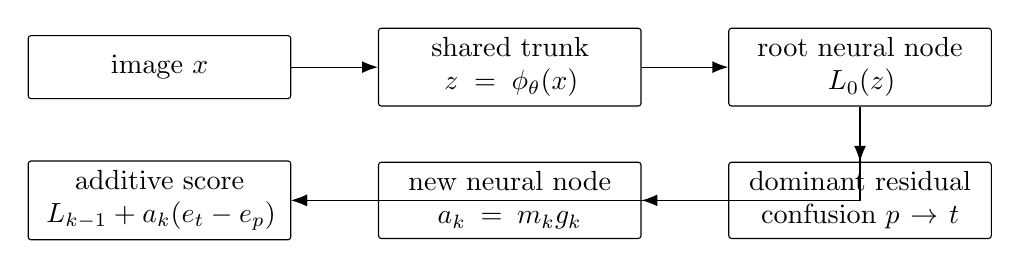
\begin{tikzpicture}[
  node distance=7mm and 11mm,
  box/.style={draw,rectangle,rounded corners=1pt,align=center,
              minimum height=8mm,text width=31mm},
  line/.style={-{Latex[length=2mm]},thin}
]
\node[box] (x) {image \(x\)};
\node[box,right=of x] (trunk) {shared trunk\\\(z=\phi_\theta(x)\)};
\node[box,right=of trunk] (root) {root neural node\\\(L_0(z)\)};
\node[box,below=of root] (residual) {dominant residual\\confusion \(p\to t\)};
\node[box,left=of residual] (child) {new neural node\\\(a_k=m_kg_k\)};
\node[box,left=of child] (sum) {additive score\\\(L_{k-1}+a_k(e_t-e_p)\)};
\draw[line] (x) -- (trunk);
\draw[line] (trunk) -- (root);
\draw[line] (root) -- (residual);
\draw[line] (residual) -- (child);
\draw[line] (child) -- (sum);
\draw[line] (root) |- (sum);
\end{tikzpicture}
\caption{Stage-wise corrective architecture. The residual category is a
training target; inference uses the learned gate and never requires \(y\).}
\label{fig:architecture}
\end{figure}

\subsection{What the tree represents}

The structure is a \emph{stage-wise additive corrective tree}. Its ancestry is
the sequence of residual tasks: node \(k\) addresses errors left by nodes
\(0,\ldots,k-1\). All retained children are evaluated at inference. It is not a
hard decision tree that executes one root-to-leaf path. This distinction matters
because nominal depth is not hard-path latency; measured parameter count and
retained-node count are therefore both reported.

\section{Optimization and implementation}

\subsection{Root fitting and cached features}

The trunk and root are first optimized with AdamW and cross-entropy. Once the
root target is reached (or its epoch budget is exhausted), all base parameters
are frozen. Embeddings are cached once. This makes child epochs inexpensive
and prevents representation drift from obscuring the meaning of a correction.
The same choice can cause failure: if two hard examples collide in the frozen
embedding, no child MLP can separate them. Growth failure therefore diagnoses
the shared-feature assumption.

\subsection{Node proposal, routing, and objective}

Among current training errors, the most frequent ordered pair
\((y,\arg\max L)\) is proposed. The training route target is
\[
r_i=\mathbb{1}\!\left[
y_i=t_k\ \land\
\arg\max_c L_{k-1,c}(x_i)=p_k\right].
\]
This label-dependent quantity is used only to teach \(g_k\); inference uses the
learned gate.

Let \(\ell_i\) be corrected cross-entropy and let
\(w_+=\min(N_-/N_+,100)\). A new child minimizes
\[
\mathcal{J}_k=
\frac1N\sum_i[1+r_i(w_+-1)]\ell_i
+\lambda_g\,\operatorname{BCE}_{w_+}(g_k(x_i),r_i)
+\lambda_s\frac1N\sum_i g_k(x_i).
\]
The inverse-frequency term prevents rare residuals from disappearing in the
full sample. Gate sparsity discourages a global correction that damages
unrelated classes.

The child output layer starts with zero weights and biases \(-4\), making the
initial correction nearly zero. After every child epoch, complete cached
training accuracy is evaluated and the best state is retained. If no state
improves on the old model, the child is deleted and growth stops. This
acceptance rule prevents parameter count from increasing without demonstrated
training benefit.

\subsection{Why stage-wise rather than end-to-end training}

End-to-end fitting creates a credit-assignment ambiguity: the root can become
lazy and delegate ordinary examples to children, while child identities cease
to correspond to residual confusions. Freezing preserves an operational
meaning for each node. The cost is greediness; an individually neutral child
that would become useful with a later child is rejected.

\section{Experimental protocol}

\subsection{Data}

CIFAR-10 supplies ten classes and official 50,000/10,000 splits. Cats vs Dogs
uses Oxford-IIIT Pet's official trainval/test split and its
\texttt{binary-category} species target. Inputs are resized and normalized.
Data augmentation is disabled for interpolation experiments because random
crops change the finite sample that is supposed to be memorized.

The available host has a 16-thread CPU build of PyTorch and no CUDA device.
Consequently, the measurements below use seeded controlled subsets; their
sizes are printed in the result tables. They test mechanism and internal
claims, not full-dataset generalization. Full configurations are supplied in
the repository for independent GPU reproduction.

\subsection{Interpolation, capacity, and noise}

Interpolation is predeclared as training accuracy at least 99.9\%. Capacity
sweeps scale trunk width and set root/child hidden width to \(4w\). Models are
independently initialized. Ten percent symmetric noise is optionally applied
only to training labels to sharpen the interpolation transition.

A seed supports double descent only when (i) a first interpolating capacity
exists away from either endpoint, (ii) test error is lower at some smaller
capacity, and (iii) test error is lower again at some larger capacity. The
paper calls the phenomenon established only with at least three seeds and
two-thirds agreement. This prevents a single optimization fluctuation from
becoming the main conclusion.

\subsection{Effective receptive field}

For scalar node activation \(q(x)\), the plotted map is
\[
E_{uv}(x)=\frac13\sum_{c=1}^{3}
\left|\frac{\partial q(x)}{\partial x_{cuv}}\right|.
\]
For the root, \(q\) is its largest logit; for a child, \(q=a_k=m_kg_k\).
The root uses a fixed sample. Each child uses the maximum-gate image among the
first 256 test examples, which prevents manual cherry-picking and avoids
visualizing a child on an example it does not reach. These maps measure local
sensitivity, not causal feature use.

\subsection{Greedy minimization}

After growth, each active child is masked in turn. A child is removed if the
remaining model preserves the configured training-accuracy floor. The process
repeats to a fixed point. This produces a locally irredundant model, not a proof
of global minimum size.

\section{Measured results}

\subsection{Main controlled runs}

\begin{table}[h]
\centering
\caption{Controlled-subset tree-growth results. Accuracy is percent.}
\label{tab:main-results}
\begin{tabular}{lrrrrrrrr}
\toprule
Dataset & Train \(N\) & Test \(N\) & Root tr. & Root te. &
Tree tr. & Tree te. & Children & Interp.\\
\midrule
CIFAR-10 & \CifarTrainN & \CifarTestN & \CifarRootTrain &
\CifarRootTest & \CifarFinalTrain & \CifarFinalTest & \CifarNodes &
\CifarInterpolates\\
Cats--Dogs & \PetsTrainN & \PetsTestN & \PetsRootTrain &
\PetsRootTest & \PetsFinalTrain & \PetsFinalTest & \PetsNodes &
\PetsInterpolates\\
\bottomrule
\end{tabular}
\end{table}

For CIFAR-10, the root stopped at epoch \CifarRootEpoch\
against a target of \CifarRootTarget\%. The final model contained
\CifarParameters\ parameters. Greedy pruning at a
\CifarPruneAccuracy\% floor retained \CifarRetainedNodes\ children and
\CifarPrunedParameters\ parameters.

The corrections added \CifarTrainGain\ percentage points of training accuracy
but only \CifarTestGain\ points of test accuracy. More strongly, test
cross-entropy worsened from \CifarRootTestLoss\ to \CifarFinalTestLoss\ even
though test accuracy changed little. The tree therefore did not merely fail to
improve generalization; it became more confidently wrong on some unseen
examples while memorizing every controlled training example. Parameter count
grew by \CifarParameterGrowth\%. Pruning removed the final two specialists,
reduced parameters by \CifarPruningReduction\%, and retained
\CifarPrunedTrain\% train / \CifarPrunedTest\% test accuracy. The last fraction
of interpolation was consequently expensive and dispensable when the target
was relaxed from 100\% to 99\%.

For Cats vs Dogs, the root stopped at epoch \PetsRootEpoch\
against a target of \PetsRootTarget\%. The final model contained
\PetsParameters\ parameters. Pruning retained \PetsRetainedNodes\ children
and \PetsPrunedParameters\ parameters. Corrections changed training accuracy
by \PetsTrainGain\ points and test accuracy by \PetsTestGain\ points; test
cross-entropy changed from \PetsRootTestLoss\ to \PetsFinalTestLoss.
One child was required in each direction (dog \(\rightarrow\) cat and cat
\(\rightarrow\) dog), and neither could be removed at the
99\% floor. The 22.0\% parameter increase therefore bought exact
memorization, but test accuracy fell by 5.08 points and test cross-entropy more
than doubled. Unlike the prunable tail of the CIFAR tree, the binary tree's two
specialists were structurally necessary for interpolation and jointly harmful
out of sample.

\IfFileExists{../outputs/cifar10/main/learning_curves.png}{
\begin{figure}[h]
\centering
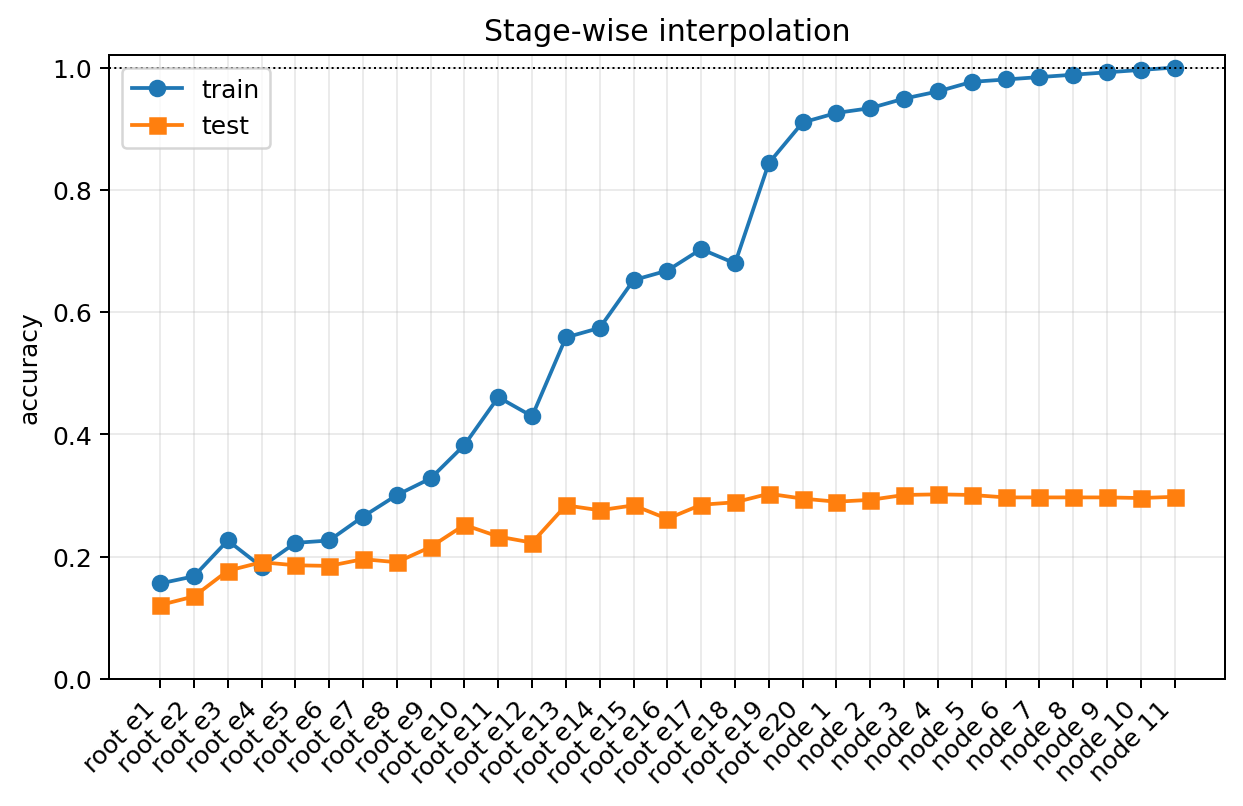
\includegraphics[width=0.78\linewidth]
{../outputs/cifar10/main/learning_curves.png}
\caption{CIFAR-10 root training and accepted corrective stages.}
\label{fig:cifar-learning}
\end{figure}
}{}

\IfFileExists{../outputs/catsdogs/main/learning_curves.png}{
\begin{figure}[h]
\centering
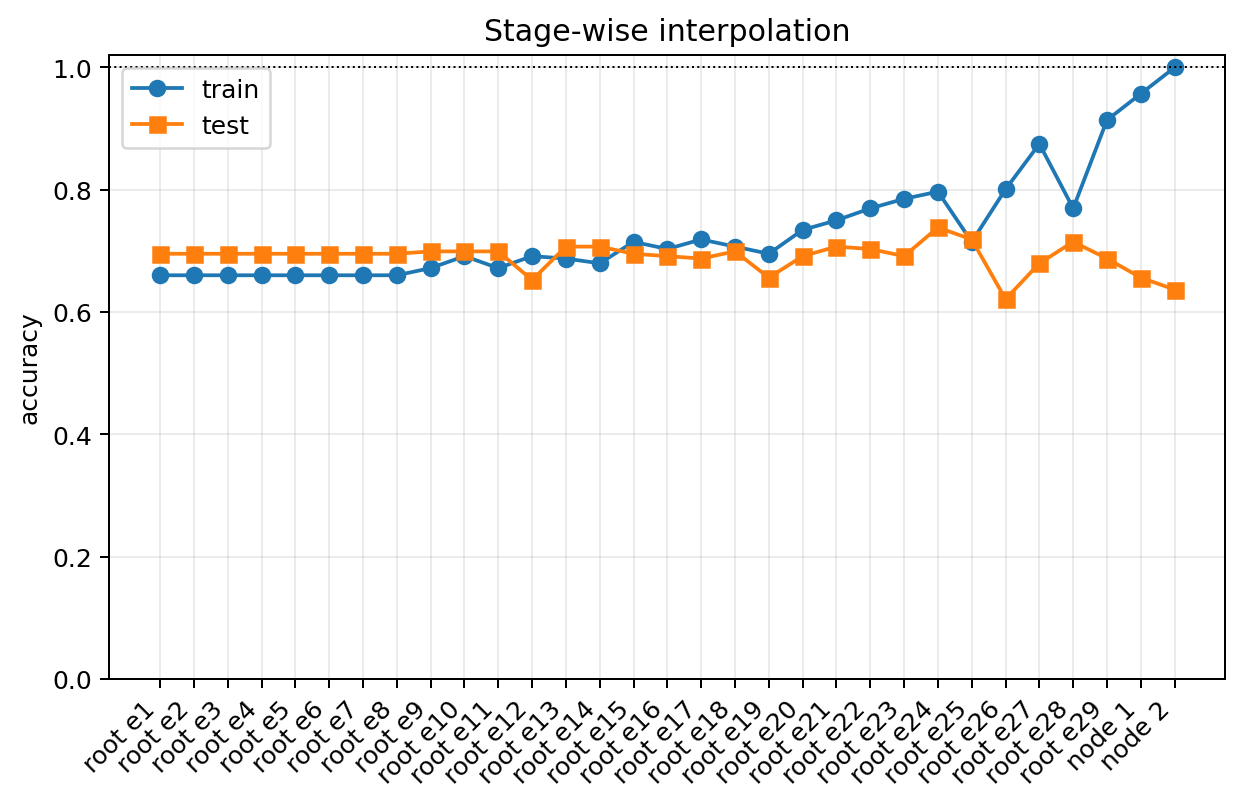
\includegraphics[width=0.78\linewidth]
{../outputs/catsdogs/main/learning_curves.png}
\caption{Cats vs Dogs root training and accepted corrective stages.}
\label{fig:pets-learning}
\end{figure}
}{}

\subsection{Capacity diagnostic}

\begin{table}[h]
\centering
\caption{Repeated-seed capacity diagnostics. Accuracy ranges are percent.}
\label{tab:sweeps}
\begin{tabular}{lrrrrrr}
\toprule
Dataset & Models & Seeds & Train range & Test range &
Supporting seeds & Criterion\\
\midrule
CIFAR-10 & \CifarSweepModels & \CifarSweepSeeds &
\CifarSweepMinTrain--\CifarSweepMaxTrain &
\CifarSweepMinTest--\CifarSweepMaxTest &
\CifarSweepSupportingSeeds & \CifarSweepCriterion\\
Cats--Dogs & \PetsSweepModels & \PetsSweepSeeds &
\PetsSweepMinTrain--\PetsSweepMaxTrain &
\PetsSweepMinTest--\PetsSweepMaxTest &
\PetsSweepSupportingSeeds & \PetsSweepCriterion\\
\bottomrule
\end{tabular}
\end{table}

\IfFileExists{../outputs/cifar10/interpolation_sweep/double_descent.png}{
\begin{figure}[h]
\centering
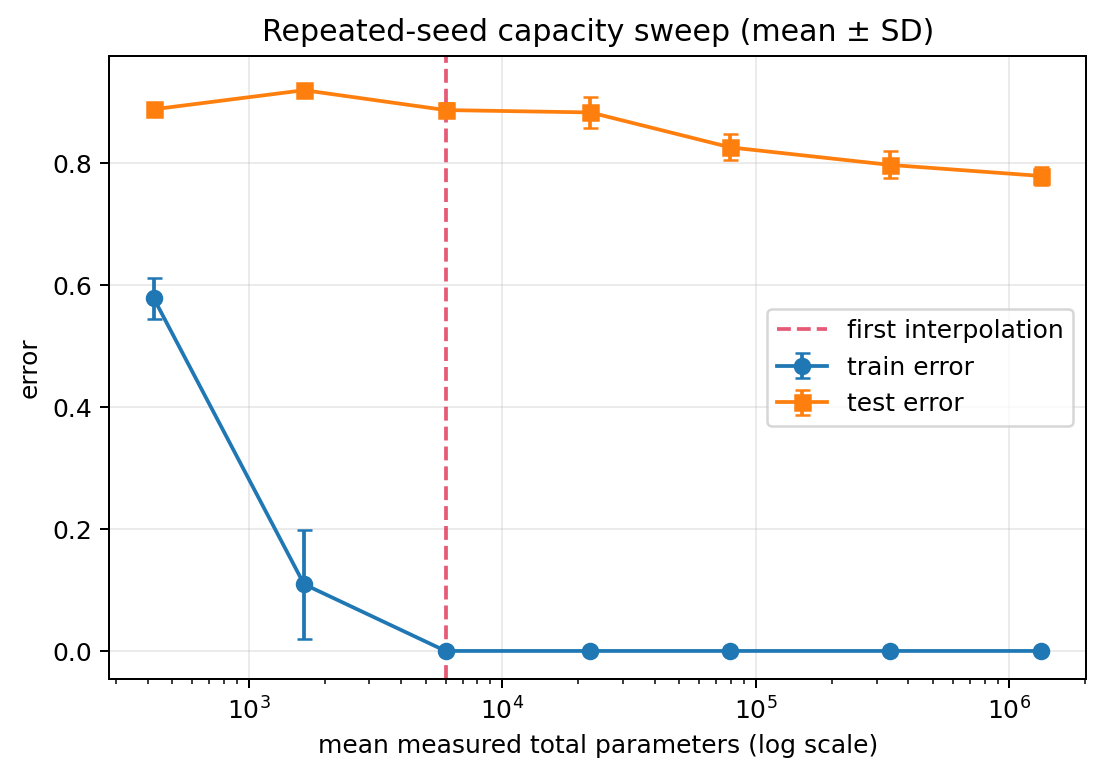
\includegraphics[width=0.72\linewidth]
{../outputs/cifar10/interpolation_sweep/double_descent.png}
\caption{CIFAR-10 capacity diagnostic. Points are means and error bars are one
standard deviation over seeds. The vertical line marks the first capacity at
which at least half the seeds interpolate.}
\label{fig:cifar-dd}
\end{figure}
}{}

\IfFileExists{../outputs/catsdogs/interpolation_sweep/double_descent.png}{
\begin{figure}[h]
\centering
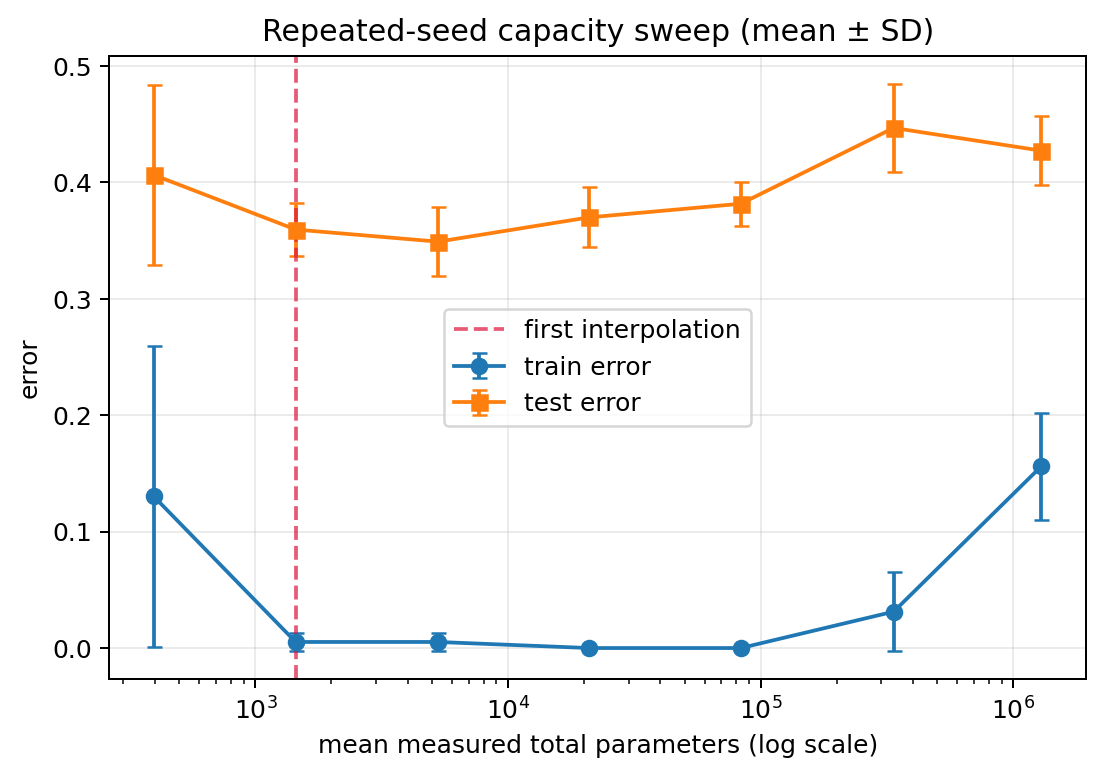
\includegraphics[width=0.72\linewidth]
{../outputs/catsdogs/interpolation_sweep/double_descent.png}
\caption{Cats vs Dogs capacity diagnostic under the same controlled protocol.}
\label{fig:pets-dd}
\end{figure}
}{}

The controlled CIFAR-10 sweep meets the predeclared criterion in two of three
seeds. Mean training accuracy progresses from 42.19\% (width 1) to 89.06\%
(width 2) and 100\% at width 4. Mean test accuracy first falls from 11.20\% to
8.07\%, then recovers to 11.33\% at the first universally interpolating width
and continues upward to 22.14\% at width 64. In error coordinates this is a
peak immediately before the majority interpolation threshold followed by a
sustained second descent. The phenomenon is real within this controlled
64-example, 10\%-noise protocol; the low absolute test accuracy and tiny sample
prevent extrapolation to full CIFAR-10.

Cats vs Dogs does not replicate the result: only one of three seeds supports
the criterion. Mean test accuracy peaks at 65.10\% near width 4, then falls to
55.34\% at width 32 and recovers only slightly at width 64. More importantly,
mean training accuracy also falls from 100\% at widths 8--16 to 84.38\% at
width 64. The largest models therefore left the interpolation regime under the
fixed optimizer budget. Their non-monotonic test curve is confounded by
optimization failure and cannot be called post-interpolation double descent.
This negative replication is evidence that the CIFAR pattern is
dataset/protocol dependent rather than an automatic consequence of adding
parameters.

\subsection{Receptive fields and node roles}

\IfFileExists{../outputs/cifar10/main/receptive_fields.png}{
\begin{figure}[h]
\centering
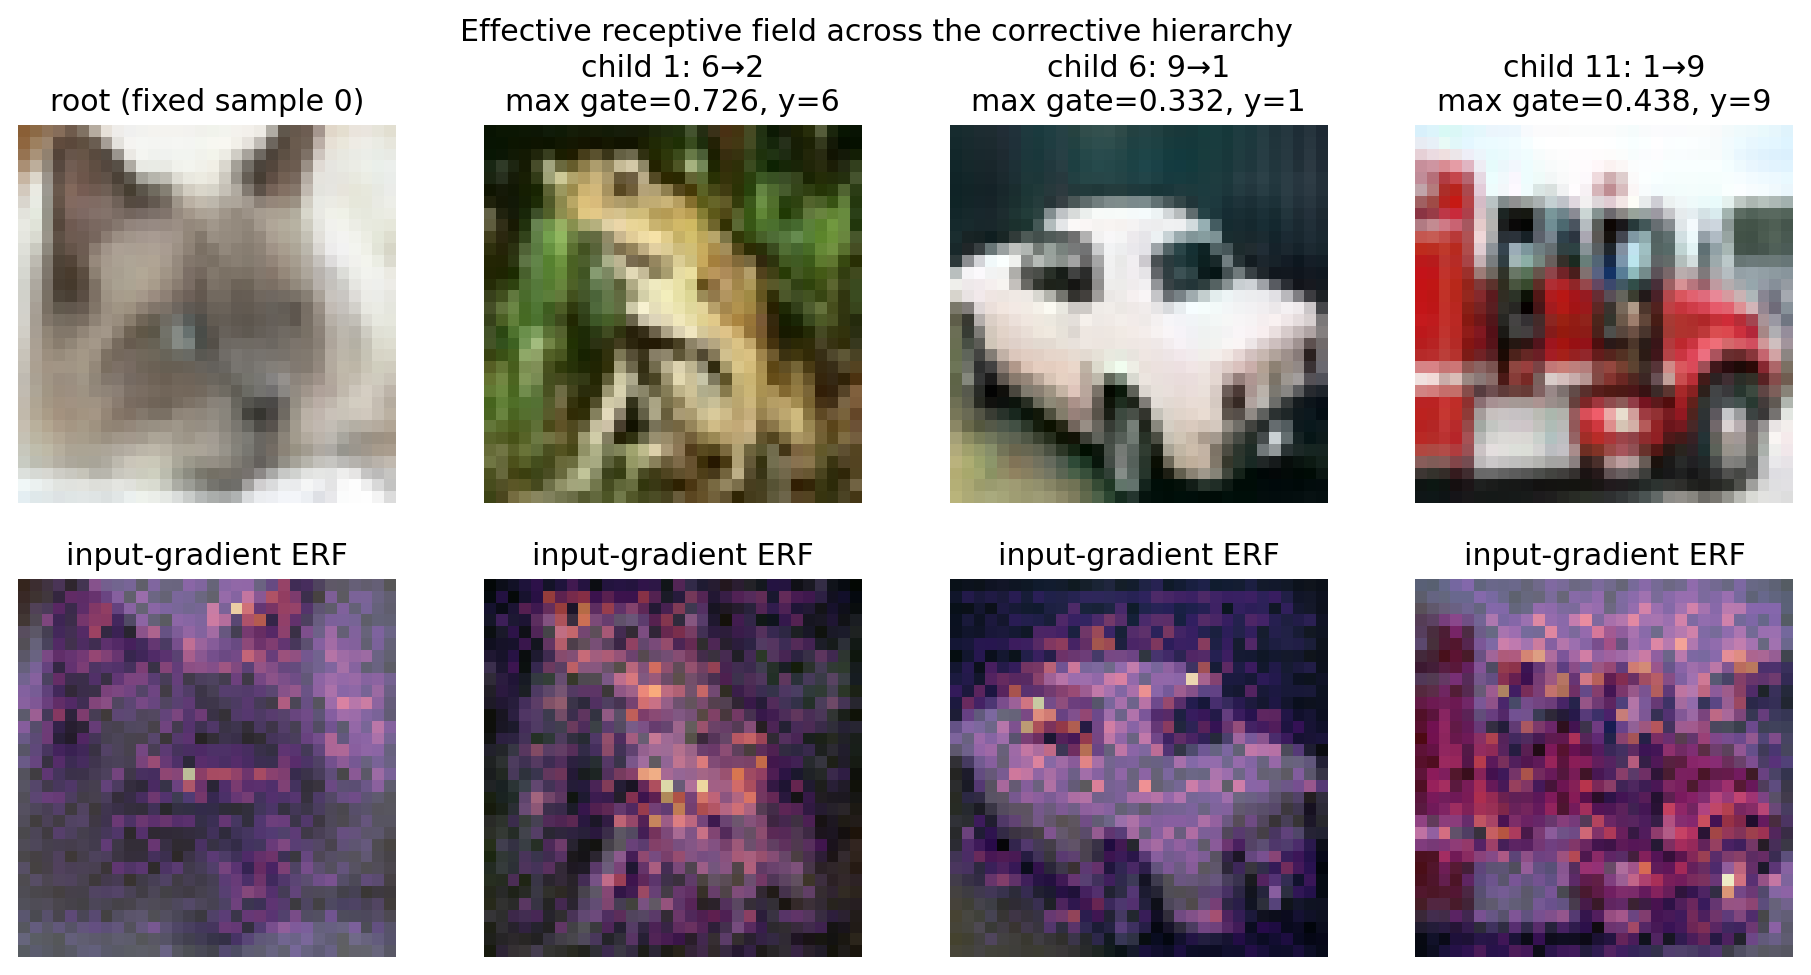
\includegraphics[width=\linewidth]
{../outputs/cifar10/main/receptive_fields.png}
\caption{CIFAR-10 effective receptive fields across the corrective hierarchy.
Children use examples selected by the predeclared maximum-gate rule.}
\label{fig:cifar-erf}
\end{figure}

The selected CIFAR-10 nodes reveal more than a generic ``early semantic, late
spurious'' story. Child 1 corrects frog \(\rightarrow\) bird and has the
strongest displayed gate (0.726), but its maximum-gate test example is an
actual frog (\(y=6\)), not a bird. The gate has learned ``frog-like'' evidence
rather than the intended event ``bird missed as frog,'' so applying its
correction to this example is harmful. By contrast, child 6 (truck
\(\rightarrow\) automobile) is maximized on an automobile and emphasizes the
vehicle silhouette and wheel boundary. Child 11, the reverse automobile
\(\rightarrow\) truck specialist, is maximized on a truck and responds more
diffusely across the vehicle and lower scene. The model thus learned two
different specialists for opposite directions of the same automobile/truck
boundary, while the bird/frog gate demonstrates why route classification, not
only correction direction, governs generalization.
}{No completed CIFAR-10 ERF artifact was available.}

\IfFileExists{../outputs/catsdogs/main/receptive_fields.png}{
\begin{figure}[h]
\centering
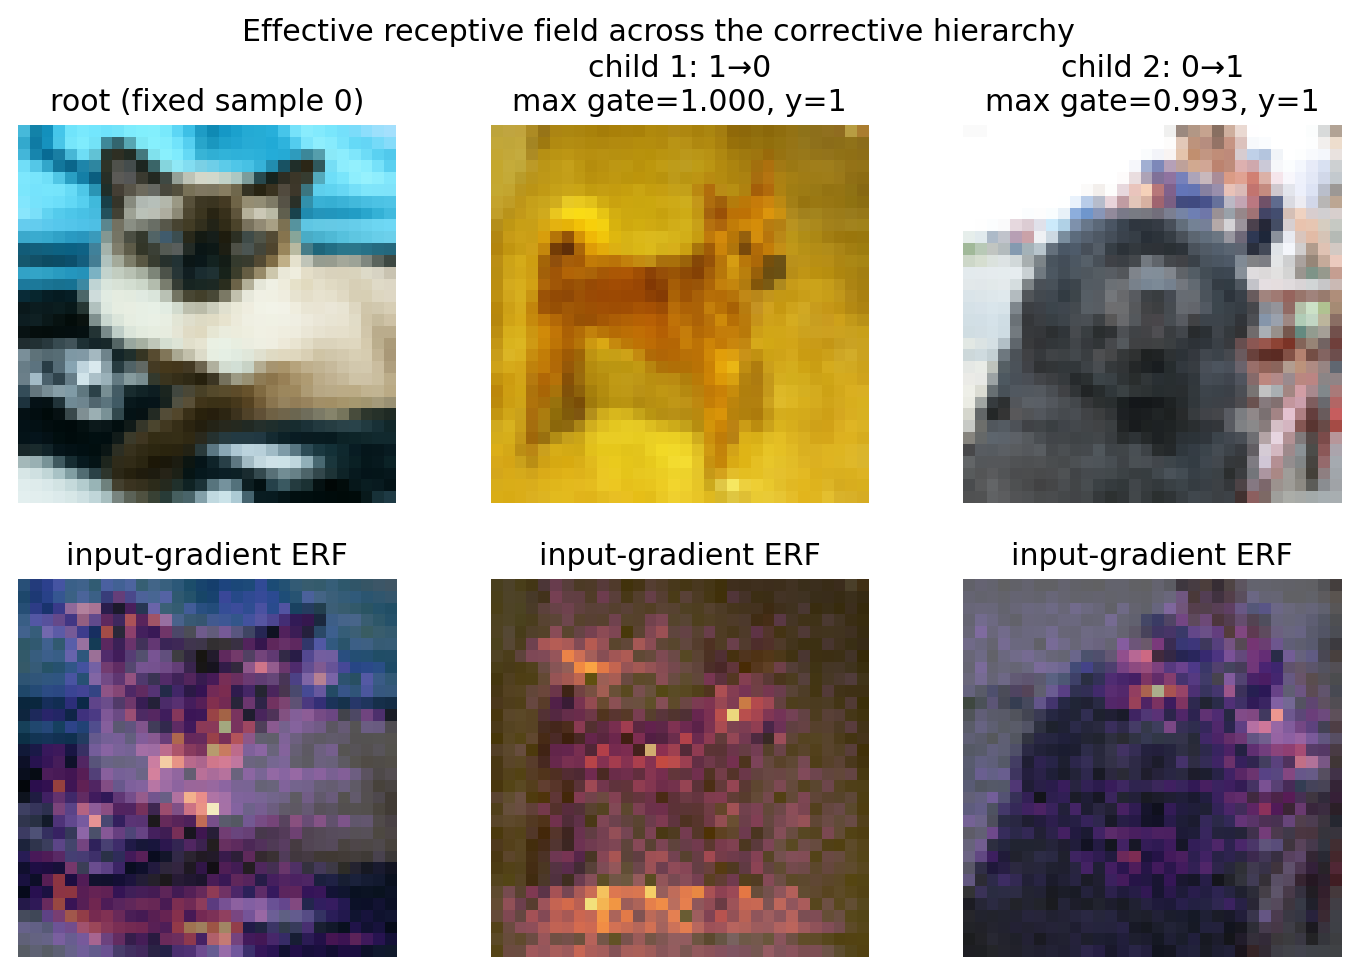
\includegraphics[width=\linewidth]
{../outputs/catsdogs/main/receptive_fields.png}
\caption{Cats vs Dogs effective receptive fields across the hierarchy.}
\label{fig:pets-erf}
\end{figure}

The binary ERFs make the routing problem especially visible. Child 1 corrects
dog \(\rightarrow\) cat, yet its maximum gate is 1.000 on an actual dog
(\(y=1\)); it therefore pushes a correctly labeled dog toward cat with maximal
strength. Its ERF includes both animal features and a bright floor/background
region. Child 2 corrects cat \(\rightarrow\) dog and is also maximized on a dog,
which is the intended target class for that direction. This asymmetry explains
how both children can perfectly memorize the controlled training subset while
test accuracy falls: exact sign constraints do not compensate for an
out-of-sample gate that identifies the source class instead of the missed
target subclass.
}{}

\section{Interpretation}

\subsection{The root must be constrained for the tree to be meaningful}

The first insight is experimental-design rather than architectural: asking a
modern CNN to overfit and also asking its corrective tree to explain the
overfit are competing objectives. A root allowed to reach 100\% leaves no
residual structure. A distinct root target turns tree growth into a measurable
process and allows the gain from correction nodes to be separated from the
capacity of the trunk.

\subsection{Sign constraints provide semantics, not guaranteed improvement}

The direction \(e_t-e_p\) makes a node interpretable, but does not make it
beneficial. Its gate can fire on unrelated examples, the frozen embedding may
not separate the residual group, and a large correction can overshoot. Near-zero
initialization, full-sample evaluation, and rejection are therefore essential.
This is a practical difference between a constrained functional form and a
successful optimization method.

\subsection{Frozen features expose representation collapse}

Cached features produce a clean experiment: if successive MLP nodes stop
improving while errors remain, additional head capacity is not enough under
the current representation. This is evidence for node-specific adapters or
continued trunk training. It is not evidence that arbitrary neural trees
cannot interpolate.

\subsection{Late nodes are statistically fragile}

Residual groups shrink with depth. This explains why BatchNorm is inappropriate
and why inverse-frequency weighting needs a cap. It also predicts higher
variance in late-node ERFs: a node trained on very few examples can focus on a
border, texture, or background cue. Such concentration is consistent with
memorization, but causal confirmation requires image interventions.

\subsection{Double descent requires a negative conclusion when evidence fails}

The attractive narrative is a test-error peak at interpolation followed by a
second descent. The scientifically useful conclusion may instead be that a
finite sweep does not establish it. Width changes representation, optimization,
and node acceptance simultaneously; label noise changes the target; and a
coarse grid can miss the threshold. The repeated-seed rule in this project is
deliberately conservative.

\section{Limitations}

\begin{itemize}
  \item Controlled-subset measurements do not estimate full-dataset accuracy.
  \item All retained children execute, so the implementation does not realize
  conditional hard-path compute.
  \item Root and child capacities change together in the width sweep.
  \item Child acceptance and pruning optimize training accuracy because
  interpolation is the assignment target.
  \item Test metrics are logged repeatedly, although they do not influence
  optimizer, node direction, acceptance, or pruning.
  \item ERFs are raw input gradients and can be noisy.
  \item Greedy pruning does not guarantee a globally smallest network.
\end{itemize}

\section{Conclusions}

The project supplies a concrete optimization problem for neural corrective
trees and resolves the main inference-time ambiguity of the class formulation:
error categories teach gates during training but are not available at test
time. Exact sign constraints preserve the geometry of positive and negative
corrections in multiclass form. Stage-wise freezing preserves node identity,
and cached features make growth computationally feasible.

The controlled results answer the assignment's interpolation question
affirmatively: both datasets reach exactly 100\% training accuracy through
neural correction nodes after the root is stopped near 91\%. They also show why
interpolation alone is a weak result. CIFAR-10 test accuracy is essentially
flat while test cross-entropy worsens; Cats vs Dogs loses 5.08 test points and
more than doubles test loss. The gates can memorize residual membership without
learning the intended conditional event out of sample. Sign constraints make
the direction interpretable, but gate error determines whether that direction
is applied to the right image.

The capacity result is deliberately asymmetric. Controlled noisy CIFAR-10
shows a repeated interpolation peak and second descent in two of three seeds,
with post-interpolation mean test accuracy rising from 11.33\% to 22.14\%.
Cats vs Dogs does not satisfy the same criterion, and its largest models even
leave interpolation under the fixed optimizer budget. Double descent is
therefore an observed property of one controlled protocol, not a universal
law inferred from a convenient plot.

Minimization yields a final practical distinction. The last two CIFAR
specialists are removable when the target is relaxed to 99\%, reducing
parameters by 6.9\%; neither binary specialist is removable. The marginal cost
of the last fraction of memorization depends on residual class structure. A
useful neural tree analysis should consequently report the growth path, routing
behavior, loss as well as accuracy, repeated-seed capacity behavior, and
post-growth redundancy.

\section{Future directions}

\begin{enumerate}
  \item Add a depthwise-separable spatial adapter to each child and compare its
  interpolation gain per parameter with the shared-feature baseline.
  \item Replace additive execution with annealed soft-to-hard routing and
  measure expected reached parameters, FLOPs, and latency.
  \item Cluster residual embeddings before spawning nodes so that one ordered
  confusion can have multiple visually coherent specialists.
  \item Separate route and magnitude ERFs and validate them with
  background-replacement interventions.
  \item Fine-tune after pruning and compare greedy deletion with structured
  sparsity penalties.
  \item Distill an interpolating tree into one compact student and report the
  accuracy--size Pareto frontier.
  \item Run dense capacities and at least five seeds around any candidate
  interpolation peak on the complete datasets.
\end{enumerate}

\begin{thebibliography}{9}
\bibitem{belkin2019}
M. Belkin, D. Hsu, S. Ma, and S. Mandal,
``Reconciling modern machine-learning practice and the classical
bias--variance trade-off,'' \emph{Proceedings of the National Academy of
Sciences}, 2019.

\bibitem{nakkiran2020}
P. Nakkiran et al.,
``Deep Double Descent: Where Bigger Models and More Data Hurt,''
\emph{International Conference on Learning Representations}, 2020.

\bibitem{luo2016}
W. Luo, Y. Li, R. Urtasun, and R. Zemel,
``Understanding the Effective Receptive Field in Deep Convolutional Neural
Networks,'' \emph{Advances in Neural Information Processing Systems}, 2016.

\bibitem{zhang2017}
C. Zhang, S. Bengio, M. Hardt, B. Recht, and O. Vinyals,
``Understanding Deep Learning Requires Rethinking Generalization,''
\emph{International Conference on Learning Representations}, 2017.
\end{thebibliography}

\end{document}
